% Exercise 1, super consistent estimator.


\noindent \textbf{Given.} $(Y_i)_{1 \le i \le n}$ iid with $Y_i \sim \mathcal{U}[0, \theta]$ for an unknown $\theta > 0$. \\

We are asked to compare two estimators of $\theta$, the method of moments estimator $\widehat\theta_{MM} = 2 \bar Y_n$ and the maximum likelihood estimator $\widehat\theta_{ML} = \max_i Y_i$, and use the better of the two to build a confidence interval for $\theta$.

\subsection*{Part (a)}

We are given that $Y \sim \mathcal{U}[0, \theta]$ with density $f(y) = 1/\theta$ on $[0, \theta]$. We compute the expectation by direct integration:
\[
E(Y) = \int_0^\theta y \cdot \frac{1}{\theta}\, dy = \frac{\theta}{2}.
\]
Rearranging, $\theta = 2 E(Y)$. The unknown $\theta$ is exactly twice the population mean of $Y$. This identity is the bridge we use in the next part to build an estimator: any sensible estimator of $E(Y)$ doubles to an estimator of $\theta$.

\subsection*{Part (b)}

The method of moments substitutes population expectations by their sample analogues. We replace $E(Y)$ in the identity $\theta = 2 E(Y)$ from part (a) by the sample mean $\bar Y_n = n^{-1} \sum_{i=1}^n Y_i$, which gives
\[
\widehat\theta_{MM} = 2 \bar Y_n.
\]
Because $\widehat\theta_{MM} = 2 \bar Y_n$ is an affine function of $\bar Y_n$, its sampling moments follow directly from those of $\bar Y_n$ by the standard rules for affine transformations of a random variable. For the mean,
\[
E(\widehat\theta_{MM}) = E(2 \bar Y_n) = 2 E(\bar Y_n).
\]
For the variance, applying the rule $\mathrm{Var}(a X) = a^2 \mathrm{Var}(X)$ with $a = 2$,
\[
\mathrm{Var}(\widehat\theta_{MM}) = \mathrm{Var}(2 \bar Y_n) = 2^2 \mathrm{Var}(\bar Y_n) = 4 \mathrm{Var}(\bar Y_n).
\]
We will use both of these in part (c) and part (g).

\subsection*{Part (c)}

We show $\widehat\theta_{MM}$ is asymptotically normal with asymptotic variance $4 V(Y)$. The only assumption needed is finite variance of $Y$, which is automatic since $Y$ takes values in the bounded interval $[0, \theta]$, so all moments exist.

The central limit theorem applies to the sample mean of iid variables with finite variance, and gives
\[
\sqrt{n}\bigl(\bar Y_n - E(Y)\bigr) \overset{d}{\longrightarrow} \mathcal{N}\bigl(0, V(Y)\bigr).
\]
We need to turn this into a statement about $\widehat\theta_{MM}$. Start from two identities derived earlier:
\[
\widehat\theta_{MM} = 2 \bar Y_n \quad \text{(part (b))}, \qquad \theta = 2 E(Y) \quad \text{(part (a))}.
\]
Subtracting the second from the first,
\[
\widehat\theta_{MM} - \theta = 2 \bar Y_n - 2 E(Y) = 2\bigl(\bar Y_n - E(Y)\bigr).
\]
Multiplying both sides by $\sqrt n$,
\[
\sqrt{n}\bigl(\widehat\theta_{MM} - \theta\bigr) = \sqrt{n} \cdot 2\bigl(\bar Y_n - E(Y)\bigr) = 2 \cdot \sqrt{n}\bigl(\bar Y_n - E(Y)\bigr).
\]
The right hand side is two times a sequence whose limit law we already have from the central limit theorem. We now invoke the following general fact: if $T_n \overset{d}{\longrightarrow} \mathcal{N}(0, \sigma^2)$ and $a$ is a real constant, then $a T_n \overset{d}{\longrightarrow} a \cdot \mathcal{N}(0, \sigma^2)$. Furthermore, multiplying a centred normal by a constant $a$ rescales its variance by $a^2$, that is $a \cdot \mathcal{N}(0, \sigma^2) = \mathcal{N}(0, a^2 \sigma^2)$. Applying this with $a = 2$, $T_n = \sqrt n (\bar Y_n - E(Y))$, $\sigma^2 = V(Y)$,
\[
\sqrt{n}\bigl(\widehat\theta_{MM} - \theta\bigr) \overset{d}{\longrightarrow} 2 \cdot \mathcal{N}\bigl(0, V(Y)\bigr) = \mathcal{N}\bigl(0, 2^2 V(Y)\bigr) = \mathcal{N}\bigl(0, 4 V(Y)\bigr).
\]
The asymptotic variance is therefore $4 V(Y)$, as claimed.

For our specific uniform model we compute $V(Y)$ directly. The second moment is
\[
E(Y^2) = \int_0^\theta y^2 \cdot \frac{1}{\theta}\, dy = \frac{1}{\theta} \cdot \frac{\theta^3}{3} = \frac{\theta^2}{3},
\]
and combined with $E(Y) = \theta/2$ from part (a),
\[
V(Y) = E(Y^2) - E(Y)^2 = \frac{\theta^2}{3} - \left(\frac{\theta}{2}\right)^2 = \frac{\theta^2}{3} - \frac{\theta^2}{4} = \frac{4 \theta^2 - 3 \theta^2}{12} = \frac{\theta^2}{12}.
\]
The asymptotic variance therefore evaluates to $4 V(Y) = 4 \cdot \theta^2/12 = \theta^2/3$. The estimator $\widehat\theta_{MM}$ is $\sqrt n$ consistent: its error shrinks at the standard rate $1/\sqrt n$.

\subsection*{Part (d)}

The alternative estimator $\widehat\theta_{ML} = \max_{1 \le i \le n} Y_i$ is natural for two reasons that we will both use later.

First, by the support of the distribution, $Y_i \le \theta$ for every $i$, so the sample maximum is always at most $\theta$ and accumulates near $\theta$ as $n$ grows. The maximum is therefore a sensible lower bound for $\theta$ that tightens with sample size.

Second, $\widehat\theta_{ML}$ is the maximum likelihood estimator. The joint density of the sample is
\[
f(y_1, \dots, y_n; \theta) = \prod_{i=1}^n \frac{1}{\theta} \mathbf{1}\{0 \le y_i \le \theta\} = \frac{1}{\theta^n}\, \mathbf{1}\bigl\{\max_i y_i \le \theta\bigr\},
\]
which is zero on the inadmissible region $\theta < \max_i y_i$. On the admissible region $\theta \ge \max_i y_i$, the indicator equals one and the likelihood reduces to
\[
L(\theta) = \theta^{-n}.
\]
Differentiating with respect to $\theta$,
\[
\frac{d L}{d \theta} = -n\, \theta^{-(n+1)} < 0 \quad \text{for every } \theta > 0,
\]
so $L$ is strictly decreasing on the admissible region. The likelihood is therefore maximised at the smallest admissible value of $\theta$, which is the smallest $\theta$ satisfying $\theta \ge \max_i y_i$, namely
\[
\widehat\theta_{ML} = \max_i Y_i.
\]
The two views agree.

\subsection*{Part (e)}

To analyse the asymptotic behaviour of $\widehat\theta_{ML}$ in part (f) we first need its full cdf. The event $\{\max_i Y_i \le x\}$ is the same as $\{Y_1 \le x \text{ and } \dots \text{ and } Y_n \le x\}$. Independence of the $Y_i$ then turns the joint probability into a product, and the marginal cdf of the uniform gives $P(Y_i \le x) = x/\theta$ for $x \in [0, \theta]$. Putting these together,
\[
P\bigl(\widehat\theta_{ML} \le x\bigr) = \prod_{i=1}^n P(Y_i \le x) = \left(\frac{x}{\theta}\right)^n
\]
for $x \in [0, \theta]$. The event is impossible for $x < 0$ and certain for $x > \theta$, so
\[
P\bigl(\widehat\theta_{ML} \le x\bigr) =
\begin{cases}
0 & \text{if } x < 0, \\
(x/\theta)^n & \text{if } x \in [0, \theta], \\
1 & \text{if } x > \theta.
\end{cases}
\]
The cdf concentrates rapidly near $\theta$ as $n$ grows. The next part turns this into a precise rate.

\subsection*{Part (f)}

We show that $Z_n = n(\theta - \widehat\theta_{ML})/\theta$ converges in distribution to $U \sim \mathrm{Exp}(1)$. Following the hint in the problem, the strategy is to verify pointwise convergence of the cdf of $Z_n$ to the cdf of $\mathrm{Exp}(1)$ at every continuity point. The target cdf
\[
F(x) = \begin{cases} 0 & x < 0, \\ 1 - \exp(-x) & x \ge 0, \end{cases}
\]
is continuous on all of $\mathbb{R}$, so we need pointwise convergence at every $x$.

Consider $x < 0$ first. Since $\widehat\theta_{ML} \le \theta$ almost surely (the support argument from part (d)), $Z_n \ge 0$ almost surely, so $P(Z_n \le x) = 0 = F(x)$.

For $x \ge 0$, and $n$ large enough that $x/n \le 1$ so that $\theta(1 - x/n) \in [0, \theta]$, we first rewrite the event $\{Z_n \le x\}$ in terms of $\widehat\theta_{ML}$. Starting from the definition of $Z_n$ and rearranging step by step,
\begin{align*}
Z_n \le x
&\iff \frac{n(\theta - \widehat\theta_{ML})}{\theta} \le x \\
&\iff n(\theta - \widehat\theta_{ML}) \le x \theta && \text{(multiply both sides by $\theta > 0$)} \\
&\iff \theta - \widehat\theta_{ML} \le \frac{x \theta}{n} && \text{(divide both sides by $n > 0$)} \\
&\iff \widehat\theta_{ML} \ge \theta - \frac{x \theta}{n} && \text{(rearrange)} \\
&\iff \widehat\theta_{ML} \ge \theta\left(1 - \frac{x}{n}\right) && \text{(factor out $\theta$)}.
\end{align*}
Each rearrangement preserves the inequality because every multiplier is strictly positive ($\theta > 0$, $n > 0$). Taking probabilities and applying the cdf from part (e),
\begin{align*}
P(Z_n \le x)
&= P\bigl(\widehat\theta_{ML} \ge \theta(1 - x/n)\bigr) \\
&= 1 - P\bigl(\widehat\theta_{ML} < \theta(1 - x/n)\bigr) && \text{(complement)} \\
&= 1 - \left(\frac{\theta(1 - x/n)}{\theta}\right)^n && \text{(cdf from part (e))} \\
&= 1 - (1 - x/n)^n && \text{($\theta$ cancels)}.
\end{align*}
The standard analysis limit $(1 - x/n)^n \to \exp(-x)$ as $n \to \infty$ then yields
\[
P(Z_n \le x) \to 1 - \exp(-x) = F(x).
\]
Combining the two cases, $P(Z_n \le x) \to F(x)$ pointwise, so $Z_n \overset{d}{\longrightarrow} \mathrm{Exp}(1)$. \qed

This is the rate result. The error $\theta - \widehat\theta_{ML}$ shrinks at rate $1/n$ rather than the standard $1/\sqrt n$, so $\widehat\theta_{ML}$ is super consistent. Part (g) cashes this in.

\subsection*{Part (g)}

We now compare the two estimators. From part (c), $\widehat\theta_{MM}$ is $\sqrt n$ consistent with asymptotic variance $\theta^2/3$. From part (f), $\widehat\theta_{ML}$ is $n$ consistent. The contrast is therefore between rates $1/\sqrt n$ and $1/n$.

\textit{MSE for $\widehat\theta_{MM}$.} The MM estimator is unbiased:
\[
E(\widehat\theta_{MM}) = 2 E(\bar Y_n) = 2 E(Y) = 2 \cdot \frac{\theta}{2} = \theta.
\]
Combining the variance scaling from part (b) with $V(Y) = \theta^2/12$ from part (c),
\[
\mathrm{Var}(\widehat\theta_{MM}) = 4 \mathrm{Var}(\bar Y_n) = 4 \cdot \frac{V(Y)}{n} = 4 \cdot \frac{\theta^2/12}{n} = \frac{\theta^2}{3 n}.
\]
Since the bias is zero, $\mathrm{MSE}(\widehat\theta_{MM}) = \mathrm{Var}(\widehat\theta_{MM}) = \theta^2/(3 n)$.

\textit{MSE for $\widehat\theta_{ML}$.} The exact finite sample moments of $\widehat\theta_{ML}$ follow from order statistic theory. Differentiating the cdf from part (e) gives the density on $[0, \theta]$,
\[
f_{\widehat\theta_{ML}}(x) = \frac{d}{dx}\left(\frac{x}{\theta}\right)^n = \frac{n x^{n-1}}{\theta^n}.
\]
Computing the first two moments by direct integration,
\[
E(\widehat\theta_{ML}) = \int_0^\theta x \cdot \frac{n x^{n-1}}{\theta^n}\, dx = \frac{n}{\theta^n} \cdot \frac{\theta^{n+1}}{n+1} = \frac{n}{n+1}\, \theta,
\]
\[
E(\widehat\theta_{ML}^2) = \int_0^\theta x^2 \cdot \frac{n x^{n-1}}{\theta^n}\, dx = \frac{n}{\theta^n} \cdot \frac{\theta^{n+2}}{n+2} = \frac{n}{n+2}\, \theta^2,
\]
and therefore
\[
\mathrm{Var}(\widehat\theta_{ML}) = E(\widehat\theta_{ML}^2) - E(\widehat\theta_{ML})^2 = \frac{n \theta^2}{n+2} - \frac{n^2 \theta^2}{(n+1)^2} = \frac{n \theta^2}{(n+1)^2 (n+2)},
\]
after putting over a common denominator and simplifying. The bias is
\[
E(\widehat\theta_{ML}) - \theta = \frac{n \theta}{n+1} - \theta = \frac{n \theta - (n+1) \theta}{n+1} = -\frac{\theta}{n+1},
\]
so $\widehat\theta_{ML}$ is biased downward by $\theta/(n+1)$. The bias and the standard deviation both shrink at rate $1/n$, so neither dominates the other. The mean squared error decomposes as
\begin{align*}
\mathrm{MSE}(\widehat\theta_{ML})
&= \mathrm{Bias}^2 + \mathrm{Var}(\widehat\theta_{ML}) \\
&= \left(\frac{\theta}{n+1}\right)^2 + \frac{n \theta^2}{(n+1)^2 (n+2)} \\
&= \frac{\theta^2}{(n+1)^2} + \frac{n \theta^2}{(n+1)^2 (n+2)} \\
&= \frac{\theta^2}{(n+1)^2} \left[1 + \frac{n}{n+2}\right] \\
&= \frac{\theta^2}{(n+1)^2} \cdot \frac{(n+2) + n}{n+2} \\
&= \frac{\theta^2 (2 n + 2)}{(n+1)^2 (n+2)} \\
&= \frac{2 \theta^2 (n+1)}{(n+1)^2 (n+2)} \\
&= \frac{2 \theta^2}{(n+1)(n+2)}.
\end{align*}

\textit{Comparison.} The MM mean squared error $\theta^2/(3n)$ decays at rate $1/n$. The ML mean squared error $2 \theta^2 / ((n+1)(n+2))$ decays at rate $1/n^2$. At $n = 1000$ and $\theta = 1$,
\[
\mathrm{MSE}(\widehat\theta_{MM}) \approx \frac{1}{3000} \approx 3.3 \times 10^{-4}, \qquad
\mathrm{MSE}(\widehat\theta_{ML}) \approx \frac{2}{1001 \cdot 1002} \approx 2 \times 10^{-6},
\]
two orders of magnitude apart.

The ML estimator is the better estimator. The downward bias does not change the comparison because the rate gain dominates.

\subsection*{Part (h)}

We confirm the rate comparison numerically in Stata. The single sample exercise asks for $n = 1000$ draws from $\mathcal{U}[0, 1]$, with the true value $\theta = 1$. The problem text directs us to the \texttt{uniform()} function. The current Stata name for that function is \texttt{runiform()}; the two draw identical $\mathcal{U}(0, 1)$ variates, so the do file uses \texttt{runiform()} and notes the substitution in its header.

For seed \texttt{12345} the run produces $\widehat\theta_{MM} = 0.985062$ and $\widehat\theta_{ML} = 0.997823$. The absolute errors against $\theta = 1$ are $0.014938$ and $0.002177$ respectively, so $\widehat\theta_{ML}$ is closer to $\theta$ by a factor of roughly $6.9$. This agrees with the rate analysis: at $n = 1000$, $\widehat\theta_{ML}$ has typical error of order $1/n = 0.001$, while $\widehat\theta_{MM}$ has typical error of order $\sqrt{1/(3n)} \approx 0.018$.

The single sample is a point comparison. To see the rate gap visually we run $R = 1000$ independent replications of the same experiment, storing the rescaled quantities
\[
a_r = \sqrt n \bigl(\widehat\theta_{MM}^{(r)} - \theta\bigr), \qquad
b_r = n \bigl(\theta - \widehat\theta_{ML}^{(r)}\bigr)/\theta,
\]
for $r = 1, \dots, R$. The rescaling matches the two limit theorems: $a_r$ should follow $\mathcal{N}(0, 1/3)$ by part (c), and $b_r$ should follow $\mathrm{Exp}(1)$ by part (f). Empirical and theoretical moments line up to three decimal places.

\begin{center}
\begin{tabular}{lcccc}
\toprule
Quantity & Empirical mean & Empirical SD & Theoretical mean & Theoretical SD \\
\midrule
$\widehat\theta_{MM}$ & $1.000128$ & $0.017902$ & $1$ & $\sqrt{1/(3n)} \approx 0.01826$ \\
$\widehat\theta_{ML}$ & $0.999003$ & $0.000968$ & $n/(n+1) \approx 0.999$ & $\theta/n = 0.001$ \\
$a_r$ & $0.004$ & $0.566$ & $0$ & $\sqrt{1/3} \approx 0.577$ \\
$b_r$ & $0.997$ & $0.968$ & $1$ & $1$ \\
\bottomrule
\end{tabular}
\end{center}

The rescaled MM estimator has near zero mean and standard deviation close to $\sqrt{1/3}$, in line with the $\mathcal{N}(0, 1/3)$ limit from part (c). The rescaled ML estimator has mean and standard deviation both close to unity, in line with the $\mathrm{Exp}(1)$ limit from part (f). The mean of $\widehat\theta_{ML}$ also tracks the closed form $n/(n+1)$ to three decimal places, an independent check on the order statistic moments used in part (g).

\begin{figure}[h]
\centering
\begin{subfigure}[b]{0.48\textwidth}
\centering
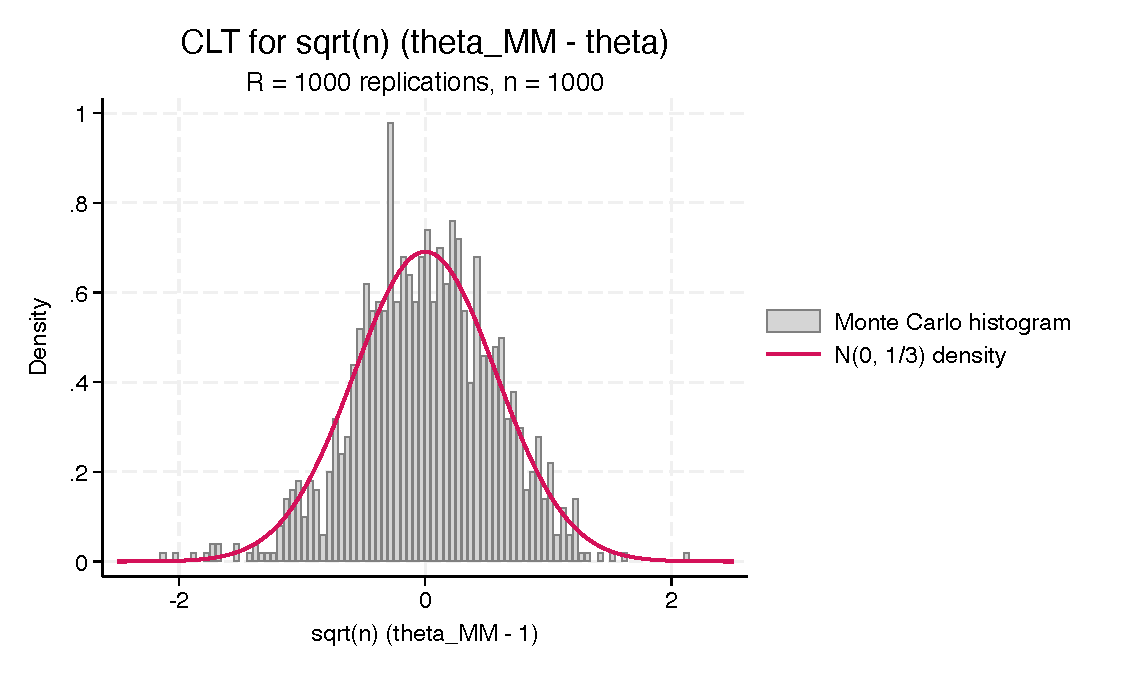
\includegraphics[width=\textwidth]{exercise1/ex1_mm_clt.pdf}
\caption{Histogram of $a_r = \sqrt n (\widehat\theta_{MM} - \theta)$ over $R = 1000$ replications, with the $\mathcal{N}(0, 1/3)$ density overlaid.}
\end{subfigure}
\hfill
\begin{subfigure}[b]{0.48\textwidth}
\centering
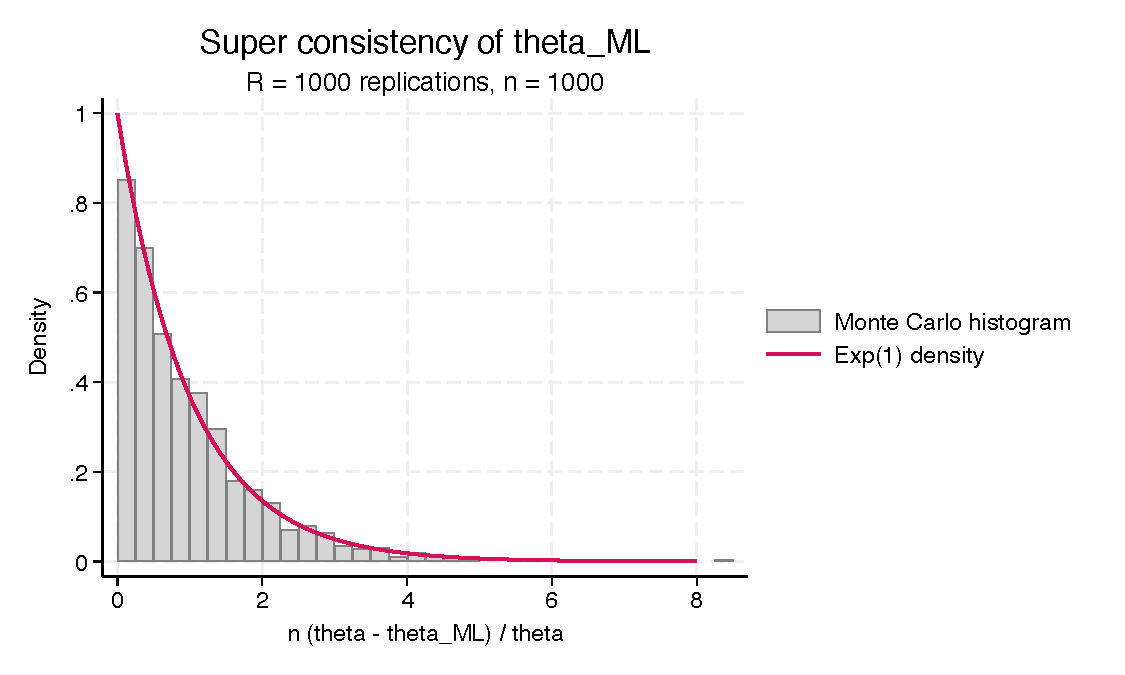
\includegraphics[width=\textwidth]{exercise1/ex1_ml_exp.pdf}
\caption{Histogram of $b_r = n(\theta - \widehat\theta_{ML})/\theta$ over $R = 1000$ replications, with the $\mathrm{Exp}(1)$ density overlaid.}
\end{subfigure}
\caption{Monte Carlo evidence for the rate gap. The left panel concentrates symmetrically around zero with spread $\sqrt{1/3}$, in line with the central limit theorem. The right panel concentrates near zero with an exponential tail of unit scale, in line with part (f).}
\label{fig:ex1_mc}
\end{figure}

The simulation confirms the analytical comparison. The MM estimator scatters around $\theta$ at scale $\theta/\sqrt{3 n}$. The ML estimator approaches $\theta$ from below at scale $\theta/n$. The visible concentration gap between the two panels of Figure~\ref{fig:ex1_mc} is the rate gap between the two limit laws.

\subsection*{Part (i)}

We now use the limit law from part (f), together with Slutsky's lemma, to build a confidence interval for $\theta$ with asymptotic coverage $1 - \alpha$.

Let $t_q = -\ln(1 - q)$ be the $q$ quantile of $\mathrm{Exp}(1)$, so that for instance $t_{0.95} = -\ln(0.05) \approx 2.996$. The proposed interval is
\[
IC(\alpha) = \left[\widehat\theta_{ML},\; \widehat\theta_{ML}\left(1 + \frac{t_{1-\alpha}}{n}\right)\right].
\]
We need to show that $P(\theta \in IC(\alpha)) \to 1 - \alpha$.

The lower endpoint takes care of itself. Since $\widehat\theta_{ML} \le \theta$ almost surely (the sample maximum is at most $\theta$), the condition $\theta \ge \widehat\theta_{ML}$ holds with probability one for every $n$. The whole question reduces to the upper endpoint, which is $\theta \le \widehat\theta_{ML}(1 + t_{1-\alpha}/n)$. Rearranging step by step,
\begin{align*}
\theta &\le \widehat\theta_{ML}\left(1 + \frac{t_{1-\alpha}}{n}\right) \\
\theta &\le \widehat\theta_{ML} + \widehat\theta_{ML} \cdot \frac{t_{1-\alpha}}{n} && \text{(distribute)} \\
\theta - \widehat\theta_{ML} &\le \widehat\theta_{ML} \cdot \frac{t_{1-\alpha}}{n} && \text{(subtract $\widehat\theta_{ML}$)} \\
\frac{n(\theta - \widehat\theta_{ML})}{\widehat\theta_{ML}} &\le t_{1-\alpha} && \text{(multiply both sides by $n/\widehat\theta_{ML} > 0$)}.
\end{align*}
Defining $W_n = n(\theta - \widehat\theta_{ML})/\widehat\theta_{ML}$, the coverage condition becomes
\[
\theta \in IC(\alpha) \;\iff\; W_n \le t_{1-\alpha},
\]
and therefore $P(\theta \in IC(\alpha)) = P(W_n \le t_{1-\alpha})$. The remaining task is the limit law of $W_n$.

Write $W_n = Z_n \cdot (\theta / \widehat\theta_{ML})$, where $Z_n = n(\theta - \widehat\theta_{ML})/\theta$ is the pivotal quantity from part (f). The first factor satisfies $Z_n \overset{d}{\longrightarrow} \mathrm{Exp}(1)$ by part (f). The second factor satisfies $\theta / \widehat\theta_{ML} \overset{P}{\longrightarrow} 1$, since $\widehat\theta_{ML} \overset{P}{\longrightarrow} \theta$ (this fact is granted in the problem and also follows from the $n$ consistency proved in part (f)) and the continuous mapping theorem applied to the map $x \mapsto \theta/x$. Slutsky's lemma in product form, namely that the product of a convergent in distribution sequence and a convergent in probability constant equals the scaled limit, then gives
\[
W_n = Z_n \cdot \frac{\theta}{\widehat\theta_{ML}} \;\overset{d}{\longrightarrow}\; \mathrm{Exp}(1) \cdot 1 = \mathrm{Exp}(1).
\]
The point $t_{1-\alpha}$ is a continuity point of the $\mathrm{Exp}(1)$ cdf, so
\[
P(\theta \in IC(\alpha)) = P(W_n \le t_{1-\alpha}) \;\longrightarrow\; P\bigl(\mathrm{Exp}(1) \le t_{1-\alpha}\bigr) = 1 - \alpha,
\]
where the last equality holds by definition of the quantile. This is the required asymptotic coverage. \qed

For $\alpha = 0.05$, $t_{0.95} = -\ln(0.05) \approx 2.996$, and the 95\% interval is
\[
IC(0.05) = \left[\widehat\theta_{ML},\; \widehat\theta_{ML}\left(1 + \frac{2.996}{n}\right)\right].
\]
At $n = 1000$ the interval has width about $0.003\, \widehat\theta_{ML}$. A standard $\sqrt n$ consistent estimator of $\theta$ would yield a confidence interval of width of order $1/\sqrt n \approx 0.03$, ten times wider. The narrow width is the practical payoff of super consistency.

\subsection*{Remark}

The problem closes with a wartime application of $\widehat\theta_{ML}$ to estimate German tank production from salvaged serial numbers. The setup differs only in that the $Y_i$ follow a discrete uniform on $\{1, \dots, \theta\}$ rather than a continuous one; the analogous results carry over with the obvious adjustments. The Allied statistical estimate of 255 tanks per month closely matched the post war recorded figure of 256, against the much higher 1400 produced by conventional intelligence. The same principle now applies in industrial intelligence and serial number analysis whenever items are issued sequentially.
